% !TeX root = ../Book1.tex
\begin{figure}[htbp]
	\centering
	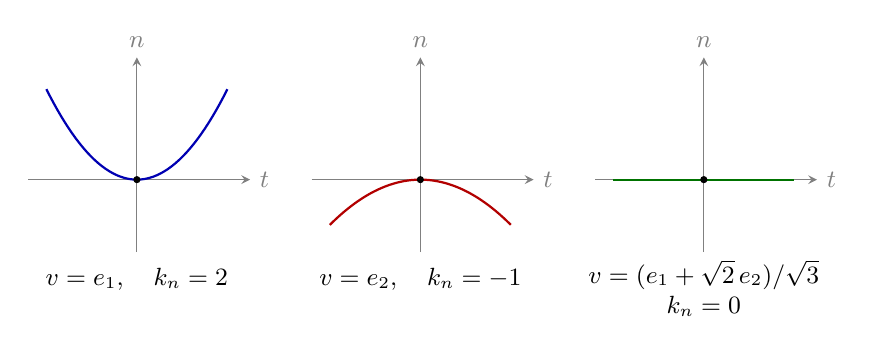
\begin{tikzpicture}[x=1.15cm,y=1.15cm,>=stealth,font=\small]
		\begin{scope}
			\draw[->,gray] (-1.2,0)--(1.25,0) node[right]{\(t\)};
			\draw[->,gray] (0,-0.8)--(0,1.35) node[above]{\(n\)};
			\draw[thick,blue!70!black,domain=-1:1,samples=50] plot(\x,{\x*\x});
			\fill (0,0) circle(1.3pt);
			\node at (0,-1.1){\(v=e_1,\quad k_n=2\)};
		\end{scope}
		\begin{scope}[xshift=3.6cm]
			\draw[->,gray] (-1.2,0)--(1.25,0) node[right]{\(t\)};
			\draw[->,gray] (0,-0.8)--(0,1.35) node[above]{\(n\)};
			\draw[thick,red!70!black,domain=-1:1,samples=50] plot(\x,{-0.5*\x*\x});
			\fill (0,0) circle(1.3pt);
			\node at (0,-1.1){\(v=e_2,\quad k_n=-1\)};
		\end{scope}
		\begin{scope}[xshift=7.2cm]
			\draw[->,gray] (-1.2,0)--(1.25,0) node[right]{\(t\)};
			\draw[->,gray] (0,-0.8)--(0,1.35) node[above]{\(n\)};
			\draw[thick,green!45!black] (-1,0)--(1,0);
			\fill (0,0) circle(1.3pt);
			\node[align=center] at (0,-1.2){\(v=(e_1+\sqrt2\,e_2)/\sqrt3\)\\\(k_n=0\)};
		\end{scope}
	\end{tikzpicture}
	\caption[鞍面在不同方向的法截线]{图像 \(z=x^2-\tfrac12y^2\) 在原点的三条法截线，各自画在由 \(v,n\) 张成的截平面内。三图的横坐标均沿单位切方向 \(v\)，纵坐标沿选定法向 \(n\)；相应截线为 \(z=t^2\)、\(z=-t^2/2\) 与 \(z=0\)。}
	\label{g1:fig:normal-sections}
\end{figure}
